\section{Предметная область}

\subsection{Задача обучения с учителем}

Обучение с учителем — один из способов машинного обучения, в ходе которого испытуемая система принудительно обучается с помощью примеров «стимул-реакция». С точки зрения кибернетики, является одним из видов кибернетического эксперимента. Между входами и эталонными выходами (стимул-реакция) может существовать некоторая зависимость, но она не известна. Известна только конечная совокупность прецедентов — пар «стимул-реакция», называемая обучающей выборкой. На основе этих данных требуется восстановить зависимость (построить модель отношений стимул-реакция, пригодных для прогнозирования), то есть построить алгоритм, способный для любого объекта выдать достаточно точный ответ. Для измерения точности ответов, так же как и в обучении на примерах, может вводиться функционал качества.

Пусть $X$ - множество описаний объектов, $Y$ - множество допустимых ответов. Существует неизвестная целевая зависимость - отображение $y: X \implies Y$, значения которой известны только на обучающей выборке 

\begin{equation}
  X_m=((x_1,y_1),...,(x_m,y_m))
\end{equation}

Требуется построить алгоритм 
\begin{equation}
  a: X \implies Y
\end{equation}
который приближал бы неизвестную целевую зависимость как на элементах выборки, так и на всём множестве $X$. 

Говорят также, что алгоритм должен обладать способностью к обобщению эмпирических фактов, или выводить общее знание (закономерность, зависимость) из частных фактов (наблюдений, прецедентов).

Данная постановка является обобщением классических задач аппроксимации функций. В классической аппроксимации объектами являются действительные числа или векторы. В реальных прикладных задачах входные данные об объектах могуть быть неполными, неточными, неоднородными, нечисловыми. Эти особенности приводят к большому разнообразию методов обучения с учителем. 

Признаком называется отображение $f: X \implies D_f$, где $D_f$- множество допустимых значений признака. Если заданы признаки $f_1,...,f_n$, то вектор
\begin{equation}
  x=(f_1(x),...,f_n(x))
\end{equation}
называется признаковым описанием объекта $x \in X$. Признаковые описания допустимо отождествлять с самими объектами. При этом множество $X=D_f1 ... D_fn$ называют признаковым пространством. 

В зависимости от множества $D_f$ признаки делятся на типы:
\begin{itemize}
  \item бинарныйы признак $D_f=(0,1)$
  \item номинальный признак $D_f$ - конечное множество
  \item порядковый признак $D_f$ - конечное упорядоченное множество
  \item количественный признак $D_f$ - множество действительных чисел.
\end{itemize}

\subsection{Задача обучения ранжированию}

\subsubsection{Классификация документов}

Классификация документов — одна из задач информационного поиска, заключающаяся в отнесении документа к одной из нескольких категорий на основании содержания документа.

Классификация может осуществляться полностью вручную, либо автоматически с помощью созданного вручную набора правил, либо автоматически с применением методов машинного обучения.

Следует отличать классификацию текстов от кластеризации, в последнем случае тексты также группируются по некоторым критериям, но заранее заданные категории отсутствуют.

Существует три подхода к задаче классификации текстов[1].

Классификация не всегда осуществляется с помощью компьютера. Например, в обычной библиотеке тематические рубрики присваиваются книгам вручную библиотекарем. Подобная ручная классификация дорога и неприменима в случаях, когда необходимо классифицировать большое количество документов с высокой скоростью.

Написании правил, по которым можно отнести текст к той или иной категории. Например, одно из таких правил может выглядеть следующим образом: "если текст содержит слова производная и уравнение, то отнести его к категории математика". Специалист, знакомый с предметной областью и обладающий навыком написания регулярных выражений, может составить ряд правил, которые затем автоматически применяются к поступающим документам для их классификации. Этот подход лучше предыдущего, поскольку процесс классификации автоматизируется и, следовательно, количество обрабатываемых документов практически не ограничено. Более того, построение правил вручную может дать лучшую точность классификации, чем при машинном обучении (см. ниже). Однако создание и поддержание правил в актуальном состоянии (например, если для классификации новостей используется имя действующего президента страны, соответствующее правило нужно время от времени изменять) требует постоянных усилий специалиста.

Третий подход основывается на машинном обучении. В этом подходе набор правил или, более обще, критерий принятия решения текстового классификатора, вычисляется автоматически из обучающих данных (другими словами, производится обучение классификатора). Обучающие данные — это некоторое количество хороших образцов документов из каждого класса. В машинном обучении сохраняется необходимость ручной разметки (термин разметка означает процесс приписывания класса документу). Но разметка является более простой задачей, чем написание правил. Кроме того, разметка может быть произведена в обычном режиме использования системы. Например, в программе электронной почты может существовать возможность помечать письма как спам, тем самым формируя обучающее множество для классификатора — фильтра нежелательных сообщений. Таким образом, классификация текстов, основанная на машинном обучении, является примером обучения с учителем, где в роли учителя выступает человек, задающий набор классов и размечающий обучающее множество.


\emph{Постановка задачи}.

Имеется множество категорий (классов, меток) $\mathfrak{C} = \{ c_1, ... , c_{ \left| \mathfrak{C} \right| } \}$.

Имеется множество документов $\mathfrak{D} = \{ d_1, ... , d_{ \left| \mathfrak{D} \right| } \}$.

Неизвестная целевая функция $\phi\colon \mathfrak{C} \times \mathfrak{D} \rightarrow \{ 0, 1 \}$.

Необходимо построить классификатор $\phi^\prime$ , максимально близкий к $\phi$.

Имеется некоторая начальная коллекция размеченных документов $\mathfrak{R} \subset \mathfrak{C} \times \mathfrak{D}$, для которых известны значения $\phi$. Обычно её делят на «обучающую» и «проверочную» части. Первая используется для обучения классификатора, вторая — для независимой проверки качества его работы.

Классификатор может выдавать точный ответ $\phi^\prime\colon \mathfrak{C} \times \mathfrak{D} \rightarrow \{ 0, 1 \}$ или степень подобия $\phi^\prime\colon \mathfrak{C} \times \mathfrak{D} \rightarrow [ 0, 1 ]$.

\emph{Этапы обработки}

\begin{itemize}

  \item Индексация документов. Построение некоторой числовой модели текста, например в виде многомерного вектора слов и их веса в документе. Уменьшение размерности модели.

  \item Построение и обучение классификатора. Могут использоваться различные методы машинного обучения: решающие деревья, наивный байесовский классификатор, нейронные сети, метод опорных векторов и др.

  \item Оценка качества классификации. Можно оценивать по критериям полноты, точности, сравнивать классификаторы по специальным тестовым наборам. 
\end{itemize}

\subsubsection{Ранжирование}

Обучение ранжированию — это класс задач машинного обучения с учителем, заключающихся в автоматическом подборе ранжирующей модели по обучающей выборке, состоящей из множества списков и заданных частичных порядков на элементах внутри каждого списка. Частичный порядок обычно задаётся путём указания оценки для каждого элемента (например, «релевантен» или «не релевантен»; возможно использование и более, чем двух градаций). Цель ранжирующей модели — наилучшим образом (в некотором смысле) приблизить и обобщить способ ранжирования в обучающей выборке на новые данные.

Применительно к поисковым системам, каждый список представляет собой набор документов, удовлетворяющих некоторому поисковому запросу.

Обучающая выборка состоит из выборки поисковых запросов, подмножества документов, им отвечающим, и оценок релевантности каждого документа запросу. Они могут быть подготовлены как вручную, специально натренированными людьми (оценщиками качества поиска или асессорами), так и автоматически, на основе анализа пользовательских кликов или таких средств поисковых систем, как система SearchWiki поисковой системы Google.

Задача улучшения ранжирования с использованием моделей поведения пользователей актуальна сейчас. Количество интернет документов и сайтов растет с оченьь большой скоростью, потребности пользователей меняются также очень быстро. Это ведет к быстрой смене релевантности документов, и ассессорам очень трудно проследить тенденции пользователей. Данная проблема имеет решение. Можно использовать неявную информацию о пользователях т.е. логи их поисковых запросов и кликов. Но правильное использование данной информации нетривиальная задача. Как показал ~\cite{joachims}, даже если документы отсортированы в обратном по релевантности порядке, пользователи всё равно будут нажимать на документы, которые стоят на первых местах.

Для решения данной проблемы строится математическая модель, которая обучается на тренеровачных данных. Было предложено ~\cite{ctr_improving1} добавить пользовательские данные, такие как количество кликов по URL, время проведения на странице, и т.д. в вектор признаков. 
Кроме этого, были предложены модели кликов ~\cite{ctr_improving2}, ~\cite{ccm}. В данном дипломном проекте рассматривается модель кликов, основанная на динамической байесовской сети ~\cite{dbn}.

\subsubsection{ Метрики качества ранжирования}

Существует несколько метрик, по которым оценивают и сравнивают качество работы алгоритмов ранжирования на выборке с асессорными оценками. Часто параметры ранжирующей модели стремятся подогнать так, чтобы максимизировать значение одной из этих метрик.

Примеры метрик:

\begin{itemize}
  \item Нормальная совокупная оценка(NDCG)
  \item Точность
  \item MAP
\end{itemize}

\subsubsection{Нормальная совокупная оценка}

Нормальная совокупная оценка используется для оценивания алгоритмов ранжирования. Данный вид оценки учитывает на только релевантность документа запросу, но также и его позицию в выдаче. Поэтому она достаточно точно отражает работу алгоритма.

Согласно ~\cite{ndcg_book} данная оценка вычисляется на основе Discounted Cumulative Gain. 

Discounted Cumulative Gain:

\begin{equation}
	DCG_p=\sum_{i=1}^{p}\frac{2^{{rel}_i}-1}{\log_2(i+1)}
\end{equation}

где ${rel}_i$ релевантность i-того документа, на позиции i. 

Т.к. количество ответов в запросе варьируется, то лучше считать нормализованныую общую оценку :

\begin{equation}
	{nDCG}_p=\frac{{DCG}_p}{{IDCG}_p}
\end{equation}

где ${{IDCG}_p}$ оценкка, вычисленная с выдачей, отсортированной по релевантности. При самом лучшем исходе, оцениваемая ввеличина ${{DCG}_p}$ равняется ${{IDCG}_p}$. 

\subsubsection{Точность}

В информационном поиске точность определяется как отношение числа релевантных документов, найденных информационной поисковой системой, к общему числу найденных документов:

\begin{equation}
  {Precision}=\frac{|D_{rel}\bigcap D_{retr}|}{|D_{rel}|}
\end{equation}

где $D_{rel}$ — это множество релевантных документов в базе, а $D_{retr}$ — множество документов, найденных системой. 

\subsection{Примененные алгоритмы}

В данном проекте были применены следующие алгоритмы:

\begin{itemize}
	\item Градиентный бустинг на основе слабых классификаторов для многослассовой задачи
	\item В качестве слабых классификаторов были использованы деревья решений
	\item В качестве целей(релевантностей документов для обучающей выборки) были использованы значения, найденные из логов пользователей с использованием динамимечкой байесовской сети
	\item Полученный алгоритм был оценен с помощью метрик NDCG, AUC, MAP.
\end{itemize}

\begin{figure}
  \centering
  \includegraphics[height=130mm]{images/architecture.png}
  \caption{Схематическое изображение системы\label{architecture}}
\end{figure}

Для ранжирования результатов был выбран градиентный бустинг с решающими деревьями. Основной причиной выбора стало то, что этот алгоритм работает не хуже, а иногда лучше ~\cite{cart_estimation_book} таких алгоритмов как метод опорных векторов и нейронная сеть. Кроме этого, градиентный бустинг с решающими деревьями обладает хорошей информативностью и слабым эффектом переобучения. ~\cite{cart_estimation_book}

Особенностью построения системы является то, что для хорошего рейтинга обучения необходимо достаточно большое количество данных и соответственно мощностей, чтобы вычислить эти данные. 

Структурная схема архитектуры приведена на рисунке ~\ref{architecture}

Данный дипломный проект демонстрирует построение алгоритма ранжирования использую современные технологии. Была продемонстрирована возможность использования действий пользователей для улучшения ранжирования. Также, централльный алгоритм обучения построен на основе деревьев, что позволяет построить схематический вид и интерпретировать результаты в вид, понятный для людей. 

Кроме этого, данный алгоритм позволяет построить диаграмму признаков и показать их информативность. Это позволяет оставить только те признаки, которые имеют информативность. Также можно проводить новые исследования и составлять алгоритмы для получения наилучшего вектора признаков(с наибольшей информативностью по признакам).

Задача информационного поиска специфична еще и тем, что обычные меры оценок не подходят. На рисунке ~\ref{feature-importance-picture} представлены информативности основных атрибутов, используемых для обучения алгоритма. Как видим, почти все они имеют одно и тоже значение, что делает задачу поиска довольно трудной.

\begin{figure}[h]
  \centering
  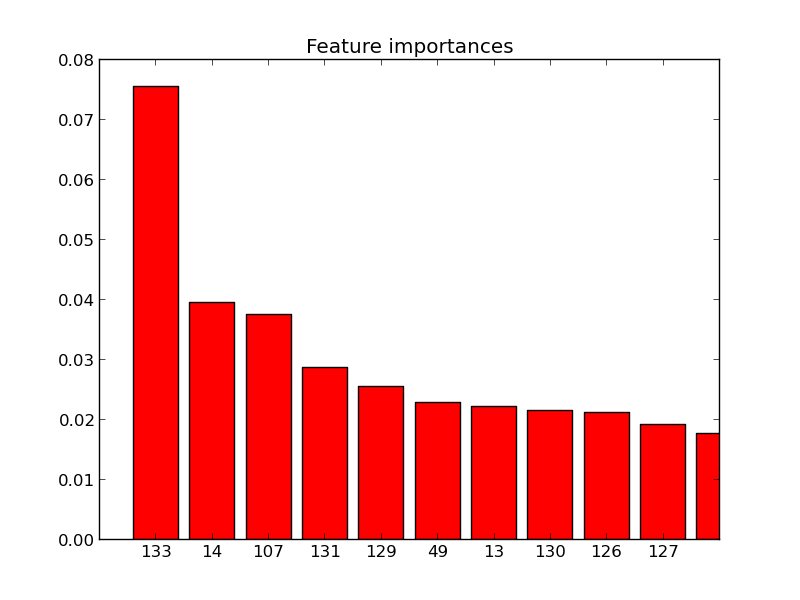
\includegraphics[width=1.0\textwidth]{images/feature_importance.png}
  \caption{Распределение  информативности образов\label{feature-importance-picture}}
\end{figure}



На рисунке ~\ref{precision-picture} приведен график зависимости точности от количества деревьев в сильном классификаторе:

\begin{figure}[h]
  \centering
  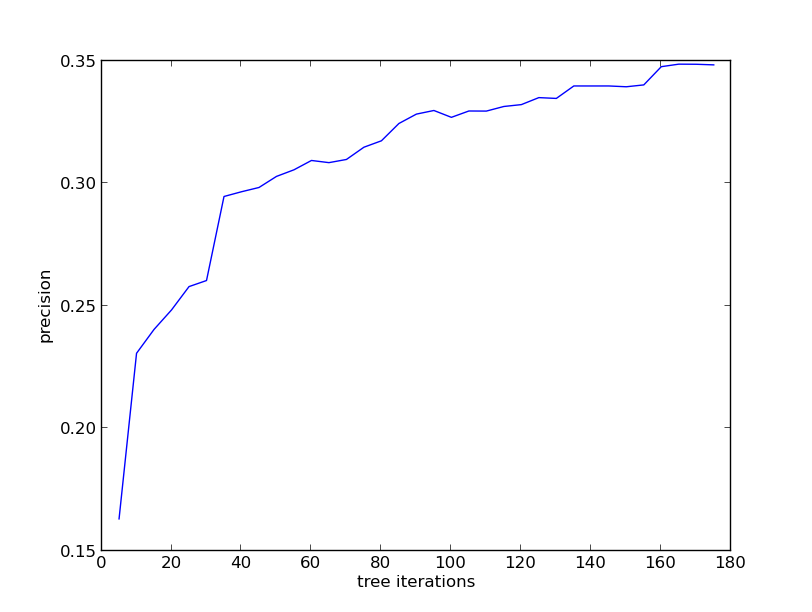
\includegraphics[width=1.0\textwidth]{images/precision_trees.png}
  \caption{График зависимости точности от количества слабых классификаторов в градиентном бустинге\label{precision-picture}}
\end{figure}

На рисунке ~\ref{ndcg-picture} приведен график зависимости нормализованной общей оценки от количества классификаторов в алгоритме бустинга. 

Как видим, с учеливением количества классификаторов растет и нормализованная общая оценка. При этом, в алгоритма бустинга не наблюдается переобучения. Поэтому данный алгоритм подходит для задачи ранжирования.

\begin{figure}[h]
  \centering
  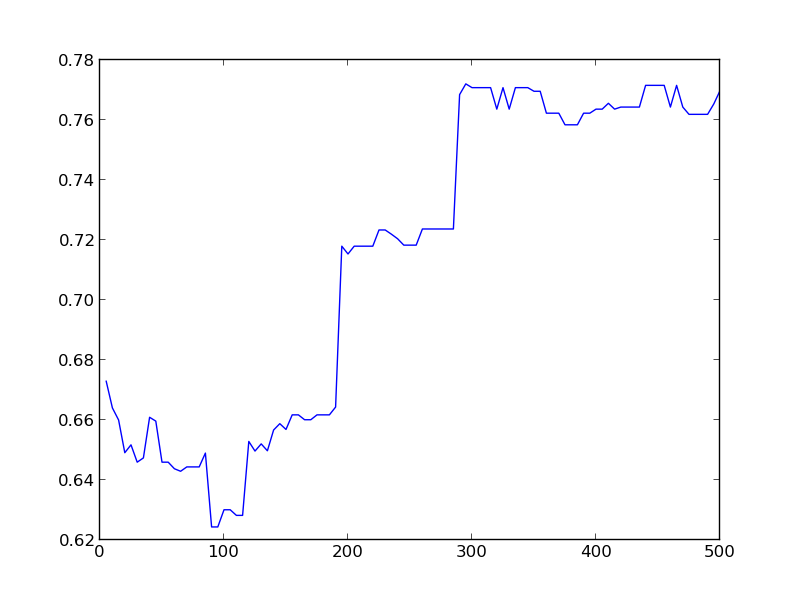
\includegraphics[width=1.0\textwidth]{images/ndcg_result1.png}
  \caption{График зависимости нормализованной общей оценки от количества слабых классификаторов\label{ndcg_result1}}
\end{figure}

